\documentclass[12pt]{article}
\usepackage[utf8]{inputenc}
\usepackage[english]{babel}

\usepackage[a4paper, margin=1in]{geometry}

\usepackage[usenames, dvipsnames]{color}

\usepackage{graphicx}
\graphicspath{ {images/} }
\usepackage{wrapfig}
\usepackage{float}

%\usepackage{minted}
%\usepackage{mdframed}
%\surroundwithmdframed{minted}

\usepackage{fancyhdr}
\pagestyle{fancy}
\fancyhf{}
\rhead{Pre-workshop Preparation}
\lhead{Workshop: Text Analysis and Word Vectors in R}
\rfoot{Page \thepage}
\lfoot{Sara J Kerr. Frankfurt - Jan 2017}

\usepackage{hyperref}
\hypersetup{
    colorlinks=true,
    linkcolor=RoyalPurple,     
    urlcolor=OliveGreen,
}
 
\urlstyle{same}


\begin{document}
\sffamily
\setlength{\parindent}{0pt}
\setlength{\parskip}{1em}

\section*{Pre-workshop Preparation}
Before taking part in the workshop it would be very helpful if you could download \textbf{R} and \textbf{R Studio}, and install the packages that will be used in the workshop as this can take a little time. The programs are free and are available for both Mac and Windows. 

I have outlined the steps needed to download the programs below.

\section{Loading R}
To download and install \textbf{R}: 

\begin{enumerate}
	\item Go to \textbf{\url{https://cran.r-project.org}} 
	\item Select the \textbf{Mac} or \textbf{Windows} download option 
	\item Follow the instructions in the sections below for your operating system
\end{enumerate}

\begin{figure}[h]
	\centering
	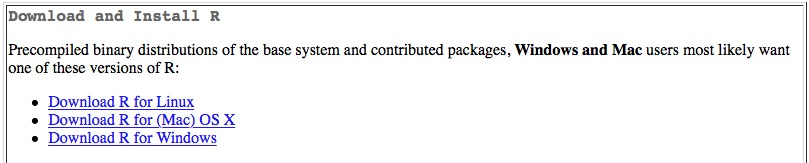
\includegraphics[width=0.75\textwidth]{downloadR.jpg}
	\caption{R Download Page}
\end{figure}

\subsection*{For Mac Users}
The following page should now be shown:

\begin{figure}[H]
	\centering
	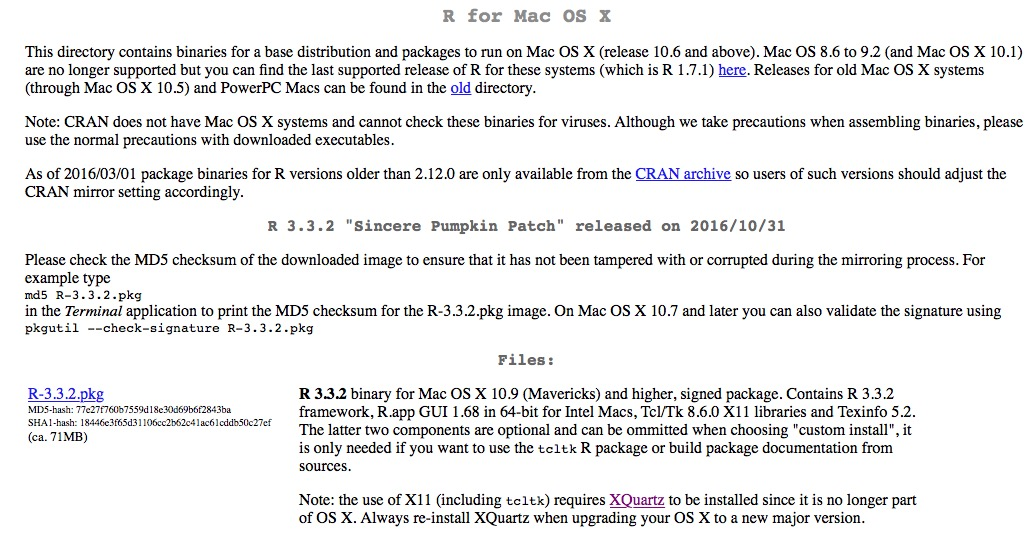
\includegraphics[width=0.75\textwidth]{macR.jpg}
	\caption{R Download Page for Mac}
\end{figure}

\textbf{Download and install R}

The download you choose depends on the operating system running on your Mac. To find out your operating system click on the \textit{Apple icon} on your menu bar and select \textit{About This Mac}.

If you are running Mavericks (OS X 10.9) or higher click on the first link to download. Double click on the downloaded .pkg file and follow the installer instructions to download. This may take a few minutes.

If you are running Snow Leopard or Mountain Lion click on the second link - if this is the case, you will not need to download XQuartz.

\textbf{Check that R has downloaded correctly}

Go to \textit{Applications} and double click on the R icon and the page below should open:

\begin{figure}[h]
	\centering
	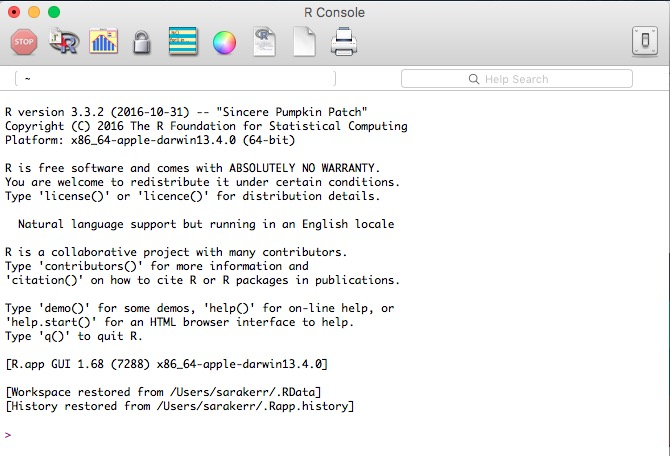
\includegraphics[width=0.75\textwidth]{rconsole.jpg}
	\caption{R Console}
\end{figure}

You can now close the R console.

If this does not work, try installing R again.

\textbf{Download and install XQuartz}

Once you have downloaded R you will also need to download the latest version of \textbf{XQuartz}. Click on the link on the R download page or go to \textbf{\url{https://www.xquartz.org}}. Follow the install instructions.

\begin{figure}[h]
	\centering
	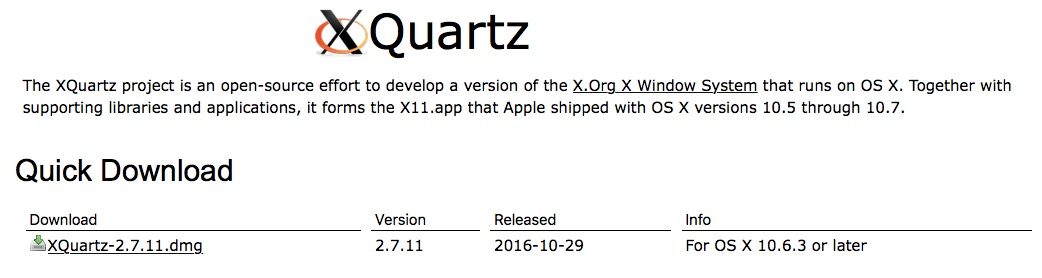
\includegraphics[width=0.75\textwidth]{xquartz.jpg}
	\caption{XQuartz Download Page}
\end{figure}

\textbf{Download Xcode and accept licence}

Finally, go to the App Store and download \textbf{Xcode}. 
 
Once it has been downloaded, go to \textit{Applications} and open Xcode by double clicking. You may be prompted to install additional elements, if so click \textit{install}. Open Xcode and accept licence. You can now close Xcode.

\subsection*{For Windows Users}
Hello, here is some text without a meaning.  This text should show what 
a printed text will look like at this place.
Testing

\section{Loading `R Studio'}
Although R can be used directly, it is easier to use it via an integrated development environment (IDE). One of the most popular IDEs for R is \textbf{R Studio}. \textbf{R Studio} is made up of four main panes which allow simultaneous access to the console, document editor, environment and help.
\begin{figure}[h]
	\centering
	\includegraphics[width=0.75\textwidth]{rstudiopanes.jpg}
	\caption{The R Studio Panes}
\end{figure}

\textbf{R Studio} can be downloaded by going to \textbf{\url{https://www.rstudio.com/products/rstudio/download/}}. Scroll down the page until you reach the heading \textit{Installers for Supported Platforms}, then select the option for your operating system. 

\begin{figure}[h]
	\centering
	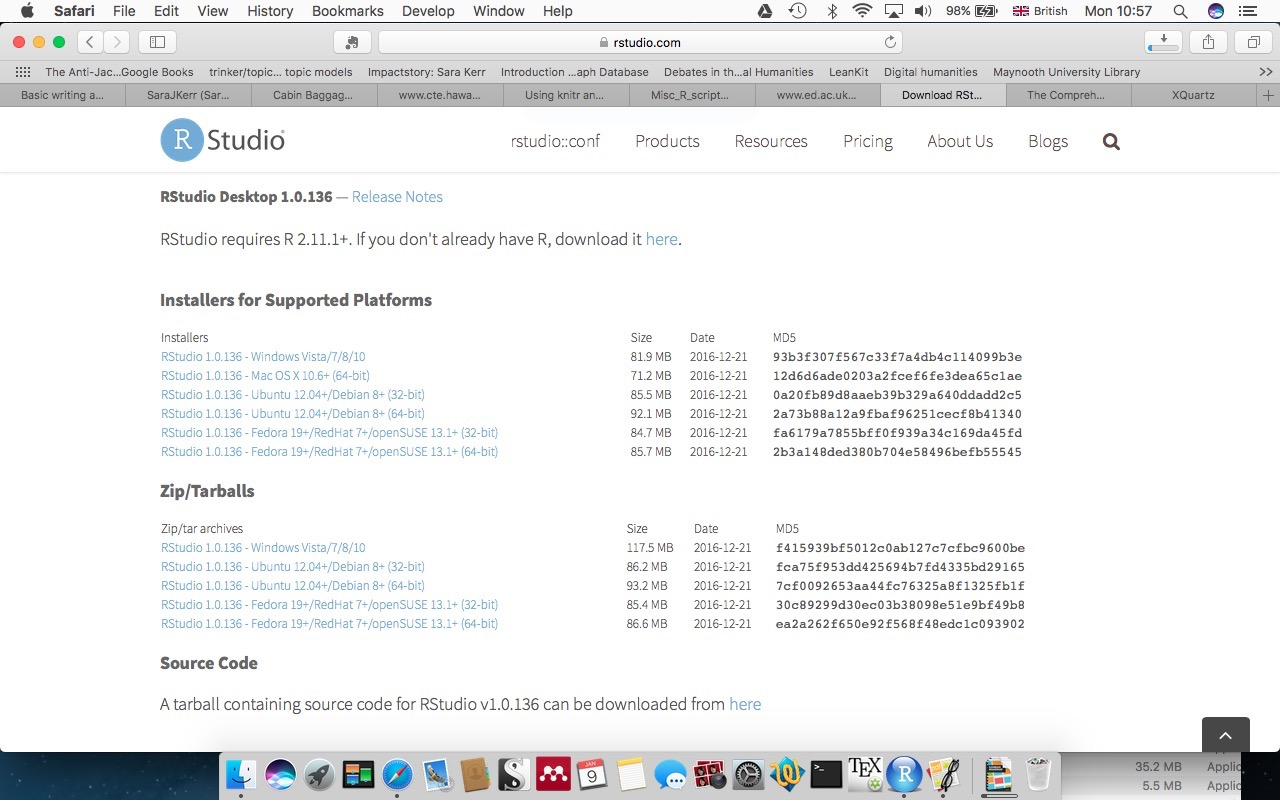
\includegraphics[width=0.75\textwidth]{rstudio.jpg}
	\caption{R Studio Download Page}
\end{figure}

The downloaded file will be .dmg for Mac or .exe for Windows. Double click and follow the installer instructions.

Check that \textbf{R Studio} has downloaded correctly by opening the program.

\textbf{Updates:} From time to time both \textbf{R} and \textbf{R Studio} are updated. This can have an impact on how packages work, especially if you are running an outdated version of \textbf{R}. Make sure you check for updates every 3--6 months.

\section{Loading the packages for the workshop}
\textbf{R} is set up with \textbf{`base' R} which includes a variety of functions and built in data sets. To improve the funtionality of \textbf{R} there is an increasingly broad range of packages available for specific uses. These can be easily added to \textbf{R} as needed. The majority of packages (almost 10000) are available via \textbf{\url{https://cran.r-project.org/web/packages/}}.

The easiest way to add packages to \textbf{R} is by using the \textit{Tools - Install Packages} option in the top menu in \textbf{R Studio}.

\begin{figure}[h]
	\centering
	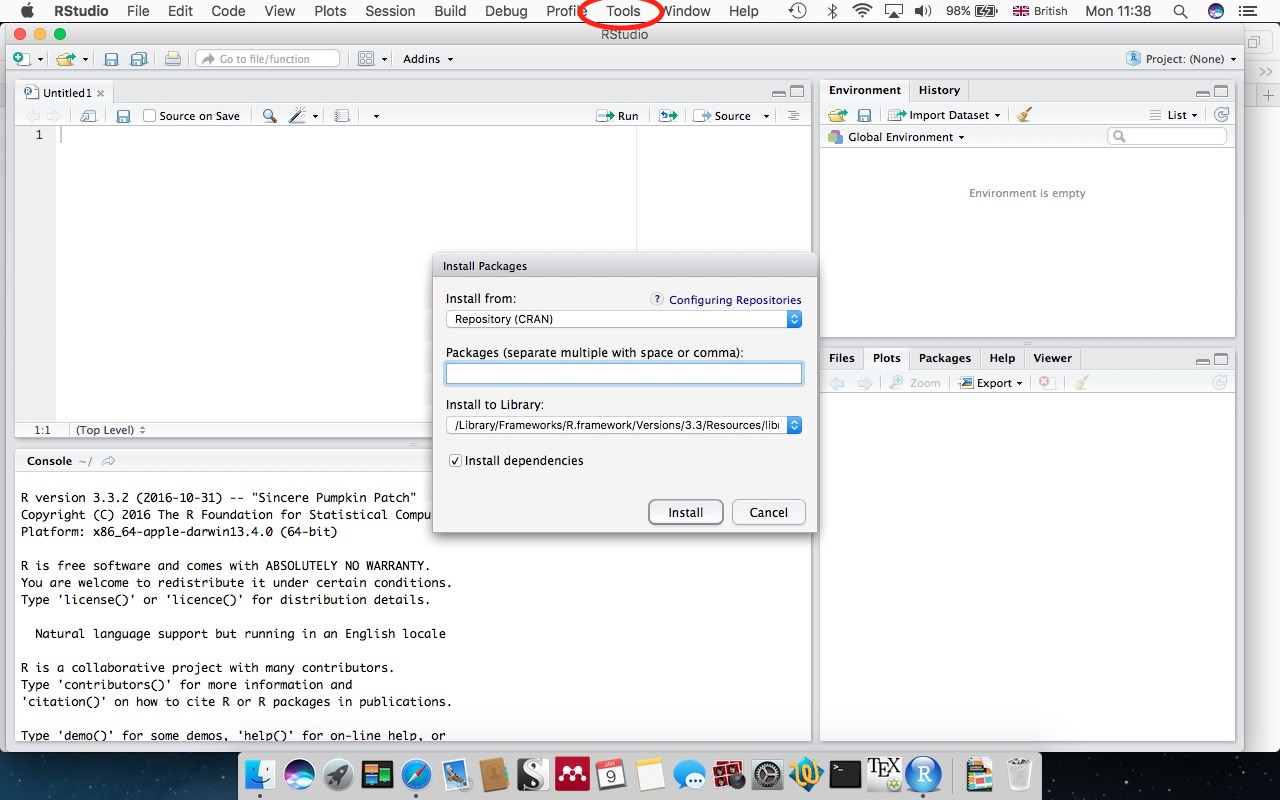
\includegraphics[width=0.75\textwidth]{installPkg.jpg}
	\caption{R Studio Install Packages}
\end{figure}

You will need to install the following \textbf{R} packages for the workshop:

It will take a little time for all the packages to install.

\section{Learning `R'}
During the workshop you will be given all the code you need to carry out the analysis. 

If you wish to get an overview of how \textbf{R} works and familiarize yourself with some of the commands \textbf{\url{https://www.datacamp.com/courses/free-introduction-to-r}} or \textbf{\url{http://tryr.codeschool.com}} give a brief practical introduction.

For a more detailed and complex introduction see \textbf{\url{https://www.r-bloggers.com/how-to-learn-r-2/}}.
 

\end{document}